\documentclass{article}
\usepackage{import}


\title{Advanced Algorithms\\Homework 02}
\author{Felix Céard-Falkenberg\\7174020}

\usepackage{../homework} % See homework.sty %
\usepackage{amsmath}
\usepackage{amssymb} 
\usepackage[utf8]{inputenc}
\usepackage{todonotes}
\usepackage{multirow}
\usepackage{multicol}
\usepackage{booktabs}
\usepackage{graphicx}
\usepackage{float}
\usepackage{subfig}
\usepackage{bbold}
\usepackage{kantlipsum}
\usepackage[bottom]{footmisc}
\usepackage{amsthm}

\newtheorem{theorem}{Theorem}


\newcommand*\dif{\mathop{}\mathrm{d}}
\newcommand{\stepandtag}{%
  \refstepcounter{equation}%
  \tag{\theequation}%
}
\newcommand{\var}{\ensuremath{\text{Var}}}
\newcommand{\group}{\ensuremath{\text{Group}}}
\newcommand{\piml}{\ensuremath{\pi_{ML}}}
\newcommand{\variance}[1]{\ensuremath{\text{\small \textcolor{gray}{$\pm #1$}}}}
% \newcommand{\variance}[1]{\text{\tiny\textcolor{gray}{$\pm$ #1}}}


\begin{document}

\section{Question 5}

\subsection{\textbf{Show that an augmenting path of capacity at least $k$ in $G_f$ can be found in $\mathcal{O}(m)$ time if such a path exists.}}
\label{question:a}


Recall that an augmenting path is a path in the residual network from the source to the sink. In our problem, we aim to find the existence of an augmenting path with capacity of at least $k$.

First, we can trivially check whether such a path is even possible in the network by checking whether $C = \max_{(u, v) \in A} c(u, v)$ is greater or equal to $k$. This can obviously be done in $\mathcal{O}(m)$ time.

Assuming that $C \geq k$, we can search for a path between the source and the sink with residual capacity of at least $k$. We can do so by using breadth-first search in the residual network. 
We assume that the residual network can be easily computed, in at most $\mathcal{O}(m)$ time.

Our algorithm works as follows: We first initialize the maximal residual capacity of each node to zero. This takes $\mathcal{O}(n)$ time. However, as the residual network can be sparse, we only need to keep track of the nodes with edges in the residual network. Therefore, the number of nodes we keep track of is at most $2m$, and therefore the initialization takes $\mathcal{O}(2m) = \mathcal{O}(m)$ time.

We then start the search from the source node $s$ and explore all adjacent nodes $u$ with edge $(s, u) \in A$ in the residual network. 
From the definition of the residual network, if an edge $(a, b)\in A$ exists, then the capacity of the edge in the residual network is greater than zero. 
For every edge $(s, u) \in A$, we update the maximal residual capacity of $u$ to the maximum of the current maximal residual capacity of $u$ and the capacity of the edge $(s, u)$. This can obviously be done in $\mathcal{O}(1)$ time.

We then repeat this process for all descendants of $s$ in the residual network. 
As at most $m$ nodes can be descendant of $s$ in the residual network, we repeat this process at most $m$ times. 

Finally, if the maximal residual capacity of the sink node is greater or equal to $k$, we have found such an augmenting path, otherwise, we can conclude that no such path exists.
As all of our operations can be done in $\mathcal{O}(m)$ time, the overall time complexity of our algorithm is $\mathcal{O}(m)$.

\begin{theorem}
    Our algorithm finds an augmenting path of capacity at least $k$, if such a path exists.
\end{theorem}
\begin{proof}
    We prove the correctness of our algorithm with a proof by contradiction.
    Let us assume that for some $k \in \mathbb{N}$, an augmenting path between a source node $s$ and a sink node $t$ with residual capacity of at least $k$ exists.

    For the sake of contradiction, let us assume that our algorithm does not find such a path, and therefore reject the existence of such a path.

    However, the breadth-first search in the residual network, starting from the source node $s$, will find the path from $s$ to $t$ in $\mathcal{O}(m)$ time.
    Because we propagate the maximal capacity of the residual flow along each investigated edge, and therefore each node, the maximal residual capacity of the sink node $t$ will be at least $k$.

    This contradicts our assumption that our algorithm does not find such a path, and therefore we can conclude that our algorithm finds an augmenting path of capacity at least $k$, if such a path exists.
\end{proof}

\subsection{\textbf{Show that the following modification of the Ford-Fulkerson algorithm returns a maximum flow in $G$.}}

We aim to show that the modification of the Ford-Fulkerson algorithm returns a maximum flow in $G$.

Recall\footnote{I'm not sure whether this has been proven in the lecture, however, it makes a lot of sense and should be easy to prove.} that a maximum flow $f$ on a graph $G$ is achieved once no more augmenting paths can be found in the residual network $G_f$.

Ignoring the runtime of the algorithm, we see that the nested while loop in lines 5--7 will repeat until no more augmenting paths can be found in the residual network $G_f$. While it is easy to show that this loop will terminate, the exact number of iterations will be determined in Question~\ref{question:d}.

By decreasing the threshold $k$ for finding the augmenting path, we ensure that, by the time the algorithm terminates, no more augmenting paths can be found in the residual network $G_f$, and therefore the algorithm returns a maximum flow in $G$.



\subsection{\textbf{Show that the capacity of a minimum cut of the residual graph $G_f$ is at most $2k \cdot m$ each time the fourth line (while $k \geq 1$) is executed.}}

After initialization of the algorithm, we have $2^{(\log C)-1} \geq k \geq 2^{\log C}$.
In the worst case, there exists an augmenting path with capacity of $C$ in the residual network $G_f$.
Therefore, we can upper-bound the capacity of each edge in the s-t cut by $2^{\lfloor \log C \rfloor + 1} = 2 \cdot 2^{\lfloor \log C \rfloor}$.
However, the total capacity of the s-t cut is dependent on the number of edges in the cut. As we can have at most $m$ edges in the cut, we can construct a graph where all $m$ edges are part of the s-t cut and all edges have capacity of $C$. Therefore, in this case, we have to upper-bound the total capacity of the s-t cut by $2 \cdot 2^{\lfloor \log C \rfloor} \cdot m = 2 \cdot k \cdot m$.

After each execution of the outer while loop, we know that the capacity of the highest edge is smaller than $2^{\lfloor \log C \rfloor - i}$, where $i\in \mathbb{N}\setminus \set{0}$ denotes the number of executions of the outer while loop.
Therefore, following the same argument as above, we can upper-bound the total capacity of the s-t cut by $2 \cdot 2^{\lfloor \log C \rfloor - i} \cdot m = 2 \cdot k \cdot m$ for each iteration of the outer while loop.





\subsection{\textbf{Prove that the algorithm can be implemented such that it runs in $\mathcal{O}(m^2 \log C)$ time.}}
\label{question:d}

In line 1, computing $C = \max_{(u, v) \in A} c(u, v)$ takes $\mathcal{O}(m)$ time.
Furthermore, the initialization of the flow $f$ to be zero at every edge takes $\mathcal{O}(m)$ time.

We remark that the while loop in line 4--9 takes at most $\mathcal{O}(\log C)$ times, as the index $k$ is decremented by a factor of 2 at each execution of the loop. As it is being initialized to $k = 2^{\lfloor\log C \rfloor}$, we know that it takes $\lfloor \log C \rfloor + 1$ divisions by 2 until $k < 1$.

Inside the while loop, another while loop is executed. Let us denote the second while loop as the inner while loop, and the first while loop as the outer while loop.

We first remark that the inner while loop checks whether an augmenting path of capacity at least $k$ exists in the residual network $G_f$. We have shown this in \ref{question:a} that this can be done in $\mathcal{O}(m)$ time.

Inside the inner while loop, updating the flow along the augmenting path takes $\mathcal{O}(|P|)$ time, with $|P|$ being the number of edges in the augmenting path. We can naturally upper-bound this by $\mathcal{O}(m)$, as in the worst case, the augmenting path contains every edge in the network.

\begin{figure}[t]
  \centering
  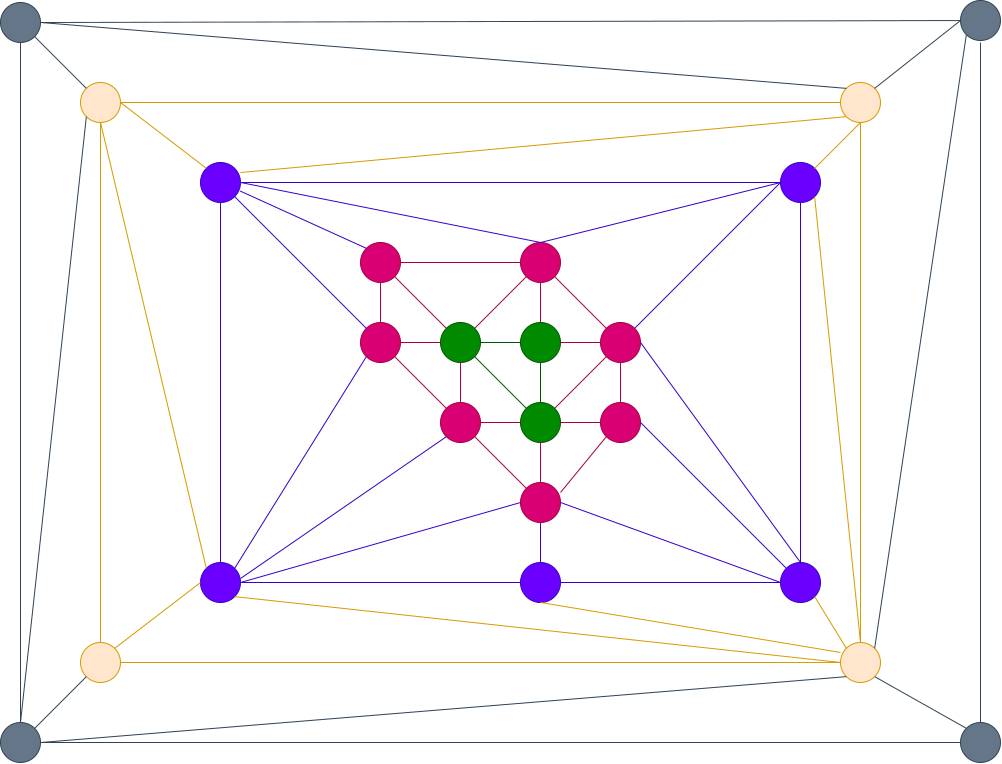
\includegraphics[width=0.75\textwidth]{graph.png}
  \caption{Example graph.}
  \label{fig:example-graph}
\end{figure}

Importantly, the inner while loop can be executed more than once. In the worst case, $\mathcal{O}(m)$ paths from the source to the sink with capacity of at least $k$ can be found. Let us illustrate this by an example. In Figure~\ref{fig:example-graph}, we depict a graph with 7 nodes (1 source, 1 sink, and 5 intermediate nodes) and 10 edges. We set the capacity of each edge in the graph to $k\in \mathbb{N}$. Therefore, in this graph, it is easy to see that there exists 5 paths from the source to the sink with equal capacity. Therefore, the inner while loop would be executed 5 times, each time finding a path with capacity of at least $k$. Therefore, the runtime of the inner while loop can be upper-bounded by $\mathcal{O}(m)$.

Note that each time the inner while loop is executed, the content of the augmenting path is distributed over the edges, and therefore the capacity of the edges on the edges in $P$ is decreased at least $k$ (the exact value depends on the path found). Nevertheless, we know that each time the inner while loop is executed, the number of paths from the source to the sink with capacity of at least $k$ in the residual network is decreased by at least one. Thus, the while loop terminates in $\mathcal{O}(\log C)$ times.

Together with the runtime of the content of the inner while loop, the runtime of the entire inner while loop is $\mathcal{O}(m^2)$. As the outer while loop is executed  $\log C$ times, the overall runtime of the algorithm is $\mathcal{O}(m^2 \log C)$.
Finally, as the initialization steps take only $\mathcal{O}(m)$ time, the overall runtime of the algorithm remains $\mathcal{O}(m^2 \log C)$.






% The augmentation of the flow along $P$ takes $\mathcal{O}(|P|)$ time, with $|P|$ being the number of edges in the augmenting path. 


\end{document}
